\section{Durchführung}

\subsection{Magnetfeld von Spulen \label{sec:mvs}}
Zunächst wird die lange Spule an das Netzgerät angeschlossen. Daraufhin werden
Strom und Spannung hochgeregelt, wobei die maximale Spannung nicht überschritten werden darf.
Mithilfe einer Longitudinalsonde wird nun die magnetische Flussdichte innerhalb und außerhalb der Spule gemessen.
Dazu soll die Sonde so justiert werden, dass das Magnetfeld auf der Achse der Spule gemessen wird.
Der Messvorgang wird für die kleine Spule wiederholt.
Der experimentelle Aufbau ist in Abbildung \ref{A1} dargestellt.
\begin{figure}
  \centering
  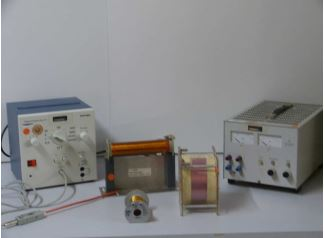
\includegraphics{Text/Bilder/Aufbau1.jpg}
  \caption{Experimenteller Aufbau \cite[4]{sample}.}
  \label{A1}
\end{figure}

\subsection{Magnetfeld von Spulenpaaren}
Ähnlich wie in Kapitel \ref{sec:mvs} wird in diesem Versuchsteil eine Helmholtz-Spule an das Netzgerät angeschlossen.
Dabei sollen beide Spulen in Reihe geschaltet werden.Die Spannung muss so gewählt werden, dass der maximal zulässige Spulenstrom
nicht überschritten wird.
Mithilfe einer transversalen Hallsonde wird die magnetische Flussdichte $\vec{B}$
für drei Spulenabstände sowohl zwischen als auch außerhalb
der Spulen gemessen.
Der experimentelle Aufbau ist in Abbildung \ref{A2} dargestellt.
\begin{figure}
  \centering
  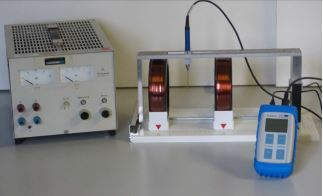
\includegraphics{Text/Bilder/Aufbau2.jpg}
  \caption{Experimenteller Aufbau \cite[5]{sample}.}
  \label{A2}
\end{figure}

\subsection{Hysteresekurve}
In diesem Versuchsteil wird das Netzgerät an eine Ringspule angeschlossen.
Erneut wird die magnetische Flussdichte $\vec{B}$ mit einer transversalen Hallsonde bestimmt.
Dazu wird hier jedoch die anliegene Spannung in regelmäßigen Abständen variiert und die Magnetische Flussdichte $\vec{B}$
mit der zugehörigen Spannung $U$ notiert.
Es werden 10-20 Messpaare aufgenommen.
Der experimentelle Aufbau ist in Abbildung \ref{A3} dargestellt.
\begin{figure}
  \centering
  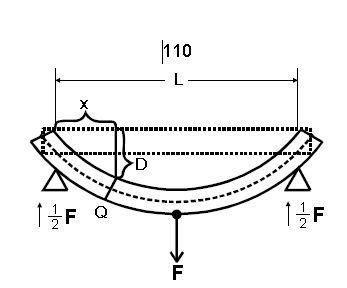
\includegraphics{Text/Bilder/Aufbau3.jpg}
  \caption{Experimenteller Aufbau \cite[5]{sample}.}
  \label{A3}
\end{figure}
